\chapter*{SISTEMAS OPERATIVOS MÓVILES ALTERNATIVOS}

\section*{Introducción}
Constantemente nos damos cuenta del gran impacto que tienen en la sociedad los sistemas operativos móviles, esto debido a la infinidad 
de posibilidades que permiten, desde conectividad inalámbrica hasta aplicaciones de desarrollo. Si bien la gran mayoría de los usuarios 
han optado al día de hoy por Android e iOS, los sistemas operativos de Google y Apple respectivamente, existen diversidad de SO móviles 
alternativos que no por ser los menos utilizados tienen capacidades limitadas. En este capítulo se hablará de esos SO alternativos, 
planteando cada una de sus características, sus fortalezas y debilidades, haciendo un recorrido desde aquellos que se han quedado en la 
historia, los que continúan siendo de agrado para algunos usuarios y de los que no tienen gran tiempo en el mercado o que están en fase 
de desarrollo y que podrían ser promesa en el campo de los sistemas operativos móviles.

\section*{Sistemas Operativos Móviles}
Los sistemas operativos móviles, también llamados SO móviles son sistemas operativos diseñados para proveer el control de distintos dispositivos móviles, tales como 
teléfonos móviles, smartphones, tablets, PDA’s (Personal Digital Assistant) y otros tales como relojes inteligentes, consolas portátiles, y dispositivos multimedia. Los SO 
móviles modernos combinan las características de los SO de los computadores y otras características, como el control de la pantalla táctil, las llamadas a celulares, 
bluetooth, Wi-Fi , GPS, cámara, reconocimiento de voz, acelerómetro, entre otros; lo que hace que estos SO estén orientados a la conectividad inalámbrica y a la multimedia.

\subsection*{Historia}
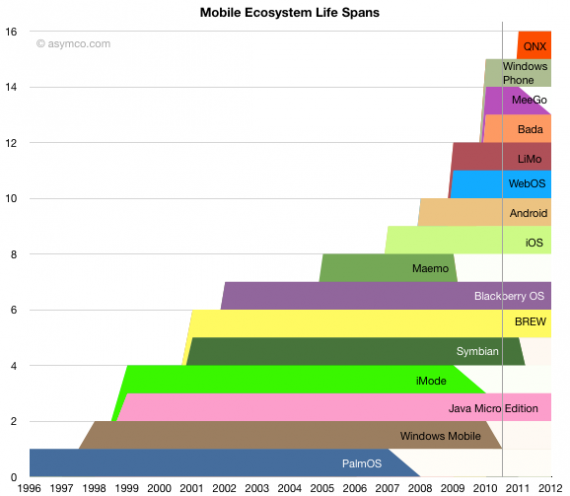
\includegraphics[scale=0.5]{img/cp01/img0101.png} 

En el vertiginoso mundo de tecnología en el que vivimos, pasamos por alto la evolución por la que han pasado los distintos avances tecnológicos para llegar a lo que son hoy 
en día, lo que no es diferente en la tecnología movil que a pesar de ser parte importante en nuestras vidas desconocemos y de paso olvidamos la importancia de los distintos 
sistemas operativos que alguna vez existieron y ya no están con nosotros y que proporcionaron las bases de los que son hoy los SO móviles reyes del mercado. Algunos de 
estos han sabido mantenerse con el tiempo, otros ya muestran debilidades y se encuentran en el final de su vida útil ya resignados a sucumbir frente a los distintos avances 
que arrasan a cualquier intento de tecnología presente en el pasado.

Y como olvidar , por ejemplo,  a Palm OS sistema operativo precursor de tantos avances tecnológicos en equipos como el Palm Pilot y el Palm Zire, entre tantos otros 
dispositivos fabricados por Palm, una empresa que hizo historia y que ahora HP, luego de adquirirla a mediados del año pasado, ha pasado a dejarla en segundo plano. Todo 
hace pensar que Palm ya no existe más.

Symbian, sistema operativo nacido el año 2001 al alero de una exitosa Nokia — por esos años líder indiscutido del mercado — vio su debut en su versión 6.0 y 6.1 
(anteriormente era llamado EPOC) en el Nokia 9210 Communicator, un equipo revolucionario en esos tiempos, era el único capaz de enviar y recibir Fax.

Casi 500.000 equipos Symbian fueron fabricados ese 2001, el año siguiente ya eran 2.100.000 equipos. En ese tiempo nació también la UI de la Serie 60, posteriormente S60. 
El resto es historia. Nokia ya le puso certificado de muerte al exitoso Symbian luego de su asociación con Microsoft.
Intel sigue intentando sacarlo a flote, MeeGo ya fue desahuciado por Nokia, tuvo una vida muy corta y ningún equipo en el mercado.
Dentro de las alternativas fuertes es todo mucho más claro, lo reyes actuales son Android, iOS y Blackberry OS, un poco más atrás vienen competidores buscando su lugar en 
la torta, Blackberry OS, Firefox OS y Windows Phone  – sucesor por excelencia del ya desaparecido Windows Mobile. El legado de algunos es innegable, Maemo dio paso a MeeGo, 
podríamos decir que Palm OS le heredó en parte su legado a webOS y Windows Mobile le cedió su puesto a Windows Phone 7.
En términos generales podríamos decir que han existido 16 plataformas principales para móviles, 10 de las cuales están aún (algunas pocas estaran, es el caso de QNX) 
compitiendo en el mercado.
Dicen que es importante conocer la historia para no volver a cometer los mismo errores, sin embargo, también es importante saber adaptarse al mercado y a las exigencias de 
los usuarios, en caso contrario se corre el riesgo de caer en el olvido y en el desuso, varios de estos sistemas operativos pueden dar cuenta de ello.

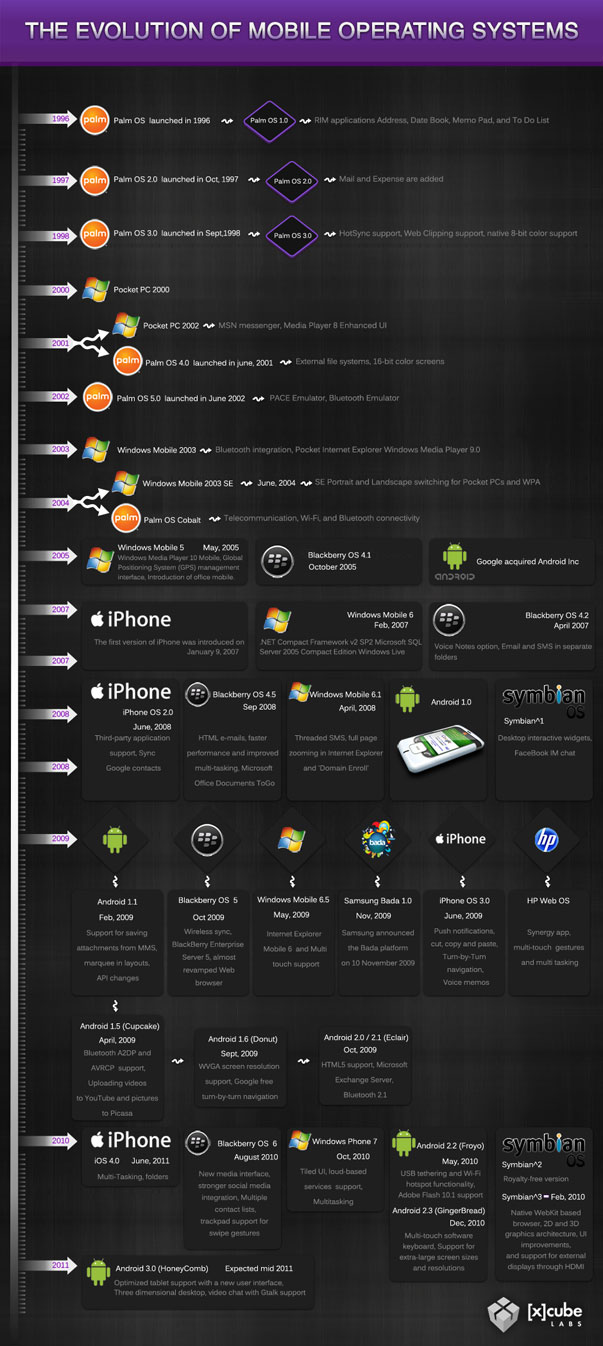
\includegraphics[scale=0.4]{img/cp01/img0102.png}

Los siguientes hitos de los sistemas operativos móviles reflejan el desarrollo en teléfonos móviles y smartphones:
\begin{itemize}
	\item 1979-1992 Los teléfonos móviles utilizan sistemas integrados para controlar la operación.
	\item 1993 El primer teléfono inteligente , el IBM Simon , posee una pantalla táctil, correo electrónico y funciones de PDA.
	\item 1996 Palm Pilot 1000 asistente personal digital (PDA) se introduce con el sistema operativo Palm OS.
	\item 1996 Se introduce el primer Windows CE para dispositivos de bolsillo.
	\item 1999 SO Nokia S40 se introduce oficialmente junto con el Nokia 7110.
	\item 2000 Symbian se convierte en el primer sistema operativo móvil moderno en un teléfono inteligente con el lanzamiento del  Ericsson R380.
	\item 2001 El Kyocera 6035 es el primer teléfono inteligente con Palm OS.
	\item 2002 Windows CE ( Pocket PC ) se introducen a los teléfonos inteligentes.
	\item 2002 BlackBerry lanza su primer teléfono inteligente.
	\item 2005 Nokia introduce Maemo OS en la primera tablet con internet, la N770.
	\item 2007 Sale al mercado el iPhone de Apple con el sistema operativo iOS, un dispositivo móvil con comunicación a internet.
	\item 2007 Se forma la Open Handset Alliance (OHA) por Google , HTC , Sony , Dell , Intel , Motorola , Samsung , LG etc.
	\item 2008 OHA lanza Android 1.0 con el HTC Dream (T-Mobile G1) como el primer teléfono con Android.
	\item 2009 Palm presenta webOS con el Palm Pre . Pero para el 2012 dispositivos con este sistema operativo se dejan de vender.
	\item 2009 Samsung anuncia el Bada OS con la introducción del Samsung S8500.
	\item 2010 Windows Phone OS es publicado, pero no es compatible con el anterior Windows Mobile OS.
	\item 2011 MeeGo el primer SO móvil Linux , combinando Maemo y Moblin , se introduce con el Nokia N9 , en colaboración con Nokia , Intel y la Fundación Linux.
	\item En septiembre de 2011 Samsung, Intel y la Fundación Linux anunciaron que sus esfuerzos pasarían de Bada y MeeGo para Tizen durante 2011 y 2012.
	\item En octubre de 2011 el proyecto de Mer se anunció, en torno a un ultra-portátil Linux + HTML5 / QML / JavaScript Core para la construcción de los productos con, 	
			derivadas de la base de código de MeeGo. 
	\item 2012 Mozilla anunció en julio de 2012, que el proyecto anteriormente conocido como "Boot to Gecko" era ahora Firefox OS contó con la colaboración de varios 		
			fabricantes de equipos móviles.
	\item 2013 Canonical anunció Ubuntu Touch , una versión de la distribución de Linux diseñada expresamente para los teléfonos inteligentes. El sistema operativo se basa 
			en el kernel Linux de Android, usando los controladores de Android, pero sin usar código Java como en Android.
	\item 2013 BlackBerry lanzó su nuevo sistema operativo para teléfonos inteligentes y tabletas, BlackBerry 10.
\end{itemize}

\subsection*{Palm OS}
Palm OS es un sistema operativo propietario destinado a dispositivos móviles, más especificamente a PDAs (Personal Digital Assistant). Palm OS comenzó su desarrollo en 1996 y Palm Inc. comenzó a licenciarlo en diciembre de 1997 con sus novedosos aparatos PalmPilot.                                               

A partir de ese momento el soporte y el desarrollo de Palm OS se disparó, llegando en enero del 2001 a tener 100.000 personas registradas en su 
red de desarrolladores trabajando en proyectos para Palm OS. Palm OS fue uno de los pioneros en el mercado de los dispositivos móviles y por 
varios años se mantuvo como uno de los mejores sistemas operativos, sobre todas las cosas por ser muy usable y simple.                                                                                                                                                                                    
                                                                                                                                                                              
A pesar de permanecer varios años en el mercado Palm OS vio el final de su vida útil en el 2008, para darle paso a un nuevo sistema operativo, WebOS, originalmente llamado Palm
WebOS, que luego fue renombrado a HP WebOS después de la compra de Palm por parte de HP.

\subsubsection*{Palm OS 1.0 (1996):}
Esta es la versión original presente en las PalmPilot 1000 y 5000, que poseen una pantalla monocroma de 160x160 soportadas por el sistema operativo, integra un entorno simple 
monotarea, la entrada de datos del usuario se genera a través del sistema de reconocimiento de escritura Graffiti, que reconoce letras y números escritas en el panel tactil de 
las PalmPilot, opcionalmente también el sistema posee un teclado virtual, un aspecto importante del sistema operativo es que no diferencia la memoria RAM del sistema de archivos 
de almacenamiento, por lo que las aplicaciones se instalan directamente en la memoria RAM y son ejecutadas desde allí.

Palm OS 1.0 integra aplicaciones PIM (Personal Information Manager) tales como Address(Libreta de direcciones), Datebook (Agenda), Memo Pad (Bloc de notas) and To do List(Lista 
de tareas), incluye ademas una Calculadora, una herramienta de seguridad para ocultar los registros de uso privado y HotSync, tecnología que permite sincronizar datos con 
computadores de mesa.

\subsubsection*{Palm OS 2.0 (1997):}
Fue lanzado en las PalmPilot Personal y Profesional. En esta versión se añaden dos nuevas aplicaciones Mail(Correo) y Expense(Gastos) además de soporte de red, HotSync por red y
soporte de retroiluminación de la pantalla.

\subsubsection*{Palm OS 3.0 (1998):}
Fue presentado con el lanzamiento de la serie Palm III. Esta versión añade comunicaciones por infrarrojo, son actualizadas las aplicaciones PIM al igual que el lanzador de 
aplicaciones, en la versión 3.2 se añade soporte de Web Clipping, con el que se puede visualizar contenido web en la pantalla del PDA, en la 3.3 el HotSync presenta mayores 
velocidades y la posibilidad de realizarlo por infrarrojo y la versión 3.5 es la primera versión que añade soporte nativo de color de 8-bits, dejando atrás las pantallas 
monocromas de los PDA’s.

\subsubsection*{Palm OS 4.0 (2001):}
Lanzado con la serie m500 de Palm. En esta versión se añade una interfaz de acceso a sistemas de archivos externos como tarjetas SD(Secure Digital), de esta manera la 
funcionalidad del sistema operativo se comporta de manera similar a los sistemas de escritorio cargando los datos de aplicación en la memoria RAM cuando se necesitan ser 
utilizados. Se introduce además un conector universal con soporte USB. El Mobile Internet Kit se incluye en el sistema operativo, este cuenta con Web Clipping,  VersaMail como 
software de correo electrónico, handPhone para gestión de SMS(Short Message Service), y Neomar como navegador WAP(Wireless Application Protocol). En esta versión de Palm OS 
también se añaden mejoras en la seguridad y en la interfaz de usuario, así como el soporte de pantallas de color de 16 bits.

Con el fin de ampliar su impacto en el mercado mundial Palm lanza una versión Palm OS 4.2 Simplified Chinese Edition dirigida especialmente al mercado chino con pleno soporte de 
Chino simplificado, de esta manera Palm OS contó con potenciales usuarios del país más poblado del mundo.

\subsubsection*{Palm OS 5 (2002):}
Implementado por primera vez en la Palm Tungsten T. Esta versión deja atrás al diseño de procesador Motorola DragonBall, al añadir soporte a la arquitectura de procesadores 
ARM(Advanced RISC Machine), arquitectura dominante actualmente en el mercado de los dispositivos móviles, proporcionando así mayores velocidades de procesamiento a los 
dispositivos Palm incluso en las aplicaciones escritas para Motorola DragonBall que pueden ser ejecutadas mediante el emulador PACE(Palm Application Compatibility Environment).

Con esta base de hardware más potente Palm mejoró considerablemente sus capacidades multimedia añadiendo soporte para Bluetooth, Wifi, y múltiples resoluciones de pantallas, 
desde 160x160 hasta 480x320, además el sistema cuenta con reproducción y grabación de sonido digital.

Al igual que en la versión 4.2 es lanzada la versión 5.3 Simplified Chinese Edition para el mercado chino.

\subsubsection*{Palm OS Cobalt (2004):}
El sucesor de Palm OS 5 fue renombrado de Palm OS 6.0 a Palm OS Cobalt. Esta versión presenta características de sistemas operativos modernos como un sistema integrado nuevo con 
multitarea y protección de memoria, gráficos modernos, nuevas características de seguridad y ajustes en el formato de archivos PIM para sincronización con Microsoft Outlook.

La versión 6.1 presenta librerías de comunicación estándar para telecomunicaciones, Wifi, Bluetooth entre otras adiciones.

\subsubsection*{El fin de Palm OS:}
La última versión de Palm OS, Palm OS Cobalt no fue adoptada para los dispositivos de los licenciatarios de Palm a pesar de incluir considerables mejoras en la versión 6.1 que 
trataba de complacer a estos licenciatarios, a partir de esto comienza el estado terminal de este sistema operativo, en el 2005 cuando todavia no habia algun dispositivo con Palm 
OS Cobalt, en una nueva estrategia PalmSource(Filial de Palm Inc para desarrollar y licenciar Palm OS, que pasaría a ser una compañía independiente en 2003) planeó portar Palm OS 
en un núcleo Linux y concentró sus esfuerzos en esta futura plataforma basada en Linux, pero con la adquisición de la PalmSource por parte de la compañía ACCESS Palm OS basado en 
linux pasa a ser Access Linux Platform, plataforma que no contó con ningún dispositivo ya que Palm Inc. no decide licenciarlo para sus dispositivos y en su lugar Palm comenzó el 
desarrollo de otros sistema operativo móvil basado en Linux llamado WebOS, dejando atrás el glorioso sistema operativo Palm OS precursor de incontables avances en la tecnología 
móvil.


\subsection*{Blackberry OS}
En distintas partes del mundo Blackberry OS tuvo un gran auge en los últimos años, una de las razones principales de este fenómeno de masificación de Blackberry en el mundo se 
debió, tal vez, a la posibilidad que permitía de comunicarse rápidamente con las demás personas a través del Blackberry Messenger (BBM), el caso de Colombia no es la excepción, 
ya que pudimos observar como Blackberry fue obteniendo gran alcance en el país haciendo surgir el fenómeno del “pineo”, una manera adoptada de referirse al pin único que 
proporciona el sistema a cada celular, con el cual las personas pueden agregarse entre sí, pero la falta de conocimiento del sistema provocó la generación de un nuevo verbo 
dedicado únicamente a Blackberry, “pinear”, que corresponde a  la acción de enviar mensajes a través del BBM. Este verbo empezó a hacer parte de la vida diaria, demostrando el 
gran auge que había originado Blackberry por medio de sus celulares, pero no todo es para siempre ya que Blackberry vió como su predominio fue disminuyendo de manera abismal con 
la aparición de nuevos dispositivos móviles de mayor gama con sistemas operativos más atractivos y con nuevas alternativas de mensajería instantánea multiplataforma, ocasionando 
una migración de de gran cantidad de usuarios a otros sistemas operativos como Android, el sistema que hoy es líder en el mundo, la gran perdida de usuarios de Blackberry los 
hizo buscar alternativas para recuperar eso que habían perdido, pero ante intentos fallidos Blackberry cedió frente a los otros SO permitiendo ahora su aplicación exclusiva de 
mensajería en las tiendas de Android y iOS. Así a pesar de que el sistema Blackberry OS ya no posee gran cantidad de usuarios como anteriormente, por medio de los sistemas 
operativos líderes, cuentan con usuarios que usan esa parte de Blackberry OS que alguna vez fue exclusiva y predominante, Blackberry Messenger.

El sistema operativo Blackberry fue desarrollado especialmente para dispositivos  móviles el cual en sus inicios solo eran disponible para teléfonos inteligentes “smartphones”. 
El sistema operativo proporciona multitarea y es compatible con dispositivos de entrada especializados que han sido adoptadas por BlackBerry Ltd.

\subsubsection*{Características:}
El SO BlackBerry en sus inicios era claramente orientado a su uso profesional como gestor de correo electrónico y agenda. Desde la cuarta versión se puede sincronizar el 
dispositivo con el correo electrónico, el calendario, tareas, notas y contactos de Microsoft Exchange Server además es compatible también con Lotus Notes y Novell GroupWise.
BlackBerry Enterprise Server (BES) proporciona el acceso y organización del email a grandes compañías identificando a cada usuario con un único BlackBerry PIN. Los usuarios más 
pequeños cuentan con el software BlackBerry Internet Service, programa más sencillo que proporciona acceso a Internet y a correo POP3 / IMAP / Outlook Web Access sin tener que 
usar BES.

Al igual que en el SO Symbian desarrolladores independientes también pueden crear programas para BlackBerry pero en el caso de querer tener acceso a ciertas funcionalidades 
restringidas necesitan ser firmados digitalmente para poder ser asociados a una cuenta de desarrollador de RIM (Research in Motion).


\subsection*{Windows Mobile}
Los primeros dispositivos que presentaron el sistema Windows Mobile datan del año 2000. Estos fueron lanzados con el nombre Pocket PC 2000, una característica de este sistema es 
que estaba basado en Windows CE 3.0.

Este sistema, está estrechamente vinculado a otros productos de la misma marca (servicios Live, Office Mobile, Internet Explorer Mobile, etc.) y cuenta con una interfaz gráfica 
de muy buena calidad, y muy similar a la de los sistemas operativos Windows.
 
Ambas cosas, ayudan a disminuir la curva de aprendizaje de los usuarios pues proveen un entorno de trabajo muy similar al que se tiene en el hogar o en la oficina.

\subsubsection*{Kernel Unificado}
\begin{itemize}
	\item El kernel de Windows CE puede manejar mas de 32000 procesos simultáneos, cada uno con 2GB de memoria virtual compartida.
	\item El filesystem soporta archivos de hasta 4GB y encriptación de dispositivos de almacenamiento externo.
\end{itemize}

\subsubsection*{Variadas Arquitecturas}
Trabaja con procesadores de arquitecturas x86, ARM, SH4 y MIPS.

\subsubsection*{Sistema de Tiempo Real}
\begin{itemize}
	\item Interrupciones anidadas.
	\item Quantums de tiempo por hilo de ejecución.
	\item 256 niveles de prioridad para hilos de ejecución.
\end{itemize}

\subsubsection*{Código Compartido}
El kernel de Windows CE es, a partir de la última versión (6.0) 100\% código compartido. Lo que comprende según Microsoft, unas 3,9 millones de líneas de código.

\subsubsection*{Características de Seguridad:}
\begin{itemize}
	\item Protección del dispositivo con contraseña.
	\item Control de acceso con contraseña al sincronizar con un PC.
	\item Aumento exponencial del tiempo de espera tras intento de acceso incorrecto.
	\item Formateo remoto del dispositivo para prevenir el acceso no autorizado a información.
	\item Cifrado del contenido de la tarjeta extraíble para prevenir el acceso no autorizado a información.
	\item Cifrado en SSL para datos transmitidos entre el dispositivo y el servidor de correo corporativo.
	\item Uso de estándar AES 128 y 256 para cifrado en comunicaciones SSL.
	\item El modo Bluetooth visible (discoverable) del dispositivo puede denegarse para prevenir la seguridad.
	\item El control de ejecución de aplicaciones permite bloquear la ejecución de aplicaciones no firmadas.
	\item Permitir o bloquear la ejecución de aplicaciones y librerías DLL no firmadas.   
\end{itemize}

Hace casi una década, este sistema se encontró en una buena posición en el mercado, ganando terreno lentamente. Más específicamente, Microsoft tuvo un total de 12\% del mercado 
entre PDAs y smartphones en el primer cuarto de 2006. En primer lugar estuvo Symbian (54,4\%) y le siguió Linux con un 21,8\%.La última versión de este sistema es la versión 6.1, 
que fue una actualización menor, desde la anterior versión estable, la 6.0.           


\subsection*{Symbian OS}
Es el resultado de una alianza entre varias empresas multinacionales de renombre en el mercado tales como Nokia, Sony Ericsson, Samsung, Siemens, Motorola y otras.Sus 
orígenes provienen del EPOC32, otro sistema operativo para dispositivos móviles, el cual pertenece a una familia de sistemas operativos que tiene sus orígenes a finales de 
1980 y principios de 1990 con el EPOC16.

Luego de unos años, más precisamente en 1997, apareció la primera versión del denominado EPOC32, que luego pasaría a llamarse Symbian OS.

\subsubsection*{Características:}
Symbian OS posee un núcleo de tiempo real. 
Es un sistema operativo con un microkernel y capacidad multithreading. 
Soporta las arquitecturas de los últimos CPU e incluso soporta hardware single-chip" o de un solo chip.                                                                                                                    

Cuenta con un sistema de archivos de alta performance.                                                                                                          

Las versiones 9.3, 9.4 y 9.5 (última versión), soporta paginación bajo demanda, una característica de la que se enorgullece mucho la compañía. La paginación bajo demanda permite 
un mejor aprovechamiento de la memoria RAM de los dispositivos a que solo se carga en memoria la "página" que se va a ejecutar.                                                                                                                   

Entre los servicios genéricos que brinda el SO, se encuentran una base de datos SQL, seguridad integrada contra malware y virus además de soporte para varias plataformas de 
desarrollo como C++, J2ME, C y MIDP 2.0.                                                                                                                   

Symbian en un tiempo fue predominante en el mercado pero en la actualidad ya ha quedado en el pasado ya que las empresas de celulares que incluían Symbian lo dejaron de lado y su 
principal marca asociada, Nokia le dió la espalda para trabajar junto con Microsoft y proporcionar en sus dispositivos el Windows Phone dejando de lado este sistema precursor de 
los sistemas operativos móviles.


\subsection*{Windows Phone}
Windows Phone es el sistema operativo moderno lanzado a finales de 2010, es sucesor de Windows Mobile, ambos desarrollados por Microsoft.. A pesar de llevar el nombre Windows, no 
son sistemas derivados de la versión de escritorio, sino nuevos sistemas diseñado específicamente para dispositivos móviles. Windows Phone esta enfocado al mercado de consumo, a 
diferencia de su antecesor que era dedicado a el mercado empresarial, este SO cuenta con una interfaz gráfica atractiva y posee los servicios propios de Microsoft, compite 
directamente con Android y iOs, pero se mantiene en la tercera posición por debajo de estos, ya que ha sido adoptado principalmente por Nokia, y muy poco por HTC, Samsung o LG, 
quienes proveen una gran cantidad de dispositivos al mercado principalmente con el sistema Android.

Windows phone demuestra modernidad en todos sus aspectos, algo que ha adoptado Microsoft también en sus sistema operativo de escritorio, Windows 8, es muy atractivo y las 
experiencia de uso es agradable, lo que demuestra que Microsoft se enfocó bastante en proveer un sistema de excelencia en diseño, y con características de alta tecnología 
actuales. La última versión de Windows Phone es la 8.1 y cuenta con Skype, Office, Skydrive, Xbox live, Internet explorer 10, entre otras, y características como Wifi, GPS, 
Bluetooth y actualizaciones OTA (Over the air), que permite actualizar el sistema desde el dispositivo sin recurrir a un computador de escritorio.


\subsection*{Firefox OS}
\subsubsection*{Comienzo del proyecto}
El 25 de julio de 2011, el Dr. Andreas Gal , Director de Investigación de la Corporación Mozilla , anunció el "Boot to Gecko" Proyecto (B2G) en la lista de correo 
mozilla.dev.platform. La propuesta de proyecto era la de "perseguir la objetivo de crear un sistema operativo completo, autónomo para la web abierta "con el fin de" encontrar las 
diferencias que mantienen a los desarrolladores Web puedan crear aplicaciones que son, en todos los sentidos - los iguales de las aplicaciones nativas creadas para el iPhone 
[iOS] ., Android y [Windows Phone 7] " El anuncio identificó estas áreas de trabajo: nuevas APIs web para exponer las capacidades del dispositivo y del sistema operativo, como el 
teléfono y la cámara, un modelo de privilegios para exponer de forma segura estos a páginas web, aplicaciones para probar estas capacidades, y el código de bajo nivel para 
arrancar en un dispositivo compatible con Android.

Esto llevó a mucha cobertura blog. De acuerdo a Ars Technica , "Mozilla dice que B2G está motivada por el deseo de demostrar que el basado en estándares Web abiertos tiene el 
potencial de ser una alternativa competitiva a la ya existente de un solo pilas de desarrollo de aplicaciones de proveedores que ofrecen los sistemas operativos móviles 
dominantes ". En 2012, el Dr. Gal se explayó sobre los objetivos de Mozilla. Se caracteriza el conjunto actual de sistemas operativos móviles como " jardines vallados " y 
presentó Firefox OS como más accesible: ". Utilizamos estándares totalmente abiertos y no hay software propietario o tecnología aplicada"  Gal también dijo que debido a que el 
pila de software es totalmente HTML5, ya hay un gran número de desarrolladores establecidos. Esta hipótesis se emplea en WebAPI de Mozilla. Estos están destinados W3C normas que 
tratan de cerrar la brecha de capacidad que existe actualmente entre los marcos nativas y web aplicaciones. El objetivo de estos esfuerzos es permitir a los desarrolladores crear 
aplicaciones usando WebAPI que ejecute en cualquier compatible con los estándares del navegador sin necesidad de reescribir sus aplicaciones para cada plataforma.

\subsubsection*{Sus tecnologías principales}
El trabajo inicial de desarrollo implica tres grandes capas de software:
Gonk - denominación plataforma para una combinación del núcleo Linux y el HAL de Android
Gecko - el motor del navegador web y aplicación de capa de servicios de tiempo de ejecución 
XULRunner - el sistema de tiempo de ejecución para cualquier cosa escrita en XUL
Gaia - un HTML5 y capa de interfaz de usuario del sistema.


\subsection*{Ubuntu Touch}
Ubuntu Touch se presentó públicamente el día 2 de enero de 2013 en la página web de Ubuntu. En la actualidad compañías como la española Bq y la china Meizu planean vender 
terminales con Ubuntu Touch durante el 2014, los cuales serán vendidos mundialmente a través de sus respectivas páginas web.

Ubuntu Touch se caracteriza por ser un sistema diseñado para plataformas móviles. Ubuntu Touch utiliza el framework Qt5 basado en la interfaz de usuario táctil y varios marcos de 
software desarrollados originalmente para Maemo y MeeGo comooFono. Además cuenta con un inicio de sesión único, utilizando libhybris, sistema que se usa con núcleos Linux 
utilizadas en Android, lo que hace que sea fácilmente portado a los últimos teléfonos inteligentes Android.

Ubuntu Touch utiliza las mismas tecnologías esenciales del Escritorio de Ubuntu, por lo que las aplicaciones diseñadas para esta plataforma pueden ser usada en ambas. Además, los 
componentes de escritorio de Ubuntu vienen con el sistema Ubuntu Touch, permitiendo que los dispositivos táctiles de Ubuntu puedan proporcionar una completa experiencia de 
escritorio cuando se conecta a un monitor externo. Los dispositivos táctiles de Ubuntu pueden estar equipados con una sesión completa de Ubuntu y pueden cambiar por completo el 
escritorio del sistema operativo cuando se conecta a una estación de acoplamiento. Si está conectado el dispositivo se pueden utilizar todas las características de Ubuntu y el 
usuario puede realizar trabajo de oficina o incluso jugar juegos en ARM mediante el dispositivo. Algunas de sus características más destacadas son:
\begin{itemize}
	\item Pantalla de inicio sin sistema de bloqueo/desbloqueo (que funciona con un nuevo sistema de gestos y se aprovecha para mostrar notificaciones).
	\item Ubuntu Touch incluye como aplicaciones centrales de medios sociales y medios de comunicación (por ejemplo, aplicaciones de Facebook,YouTube, y un lector de RSS ). Las 		
			aplicaciones estándar, tales como una calculadora, un cliente de correo electrónico, un despertador, un gestor de archivos, e incluso un terminal están incluidos 		
			también. En este momento doce o más aplicaciones principales se están desarrollando.
	\item Integración con Ubuntu One.
\end{itemize}


\section*{Otros}
\subsection*{Tizen y Meego}

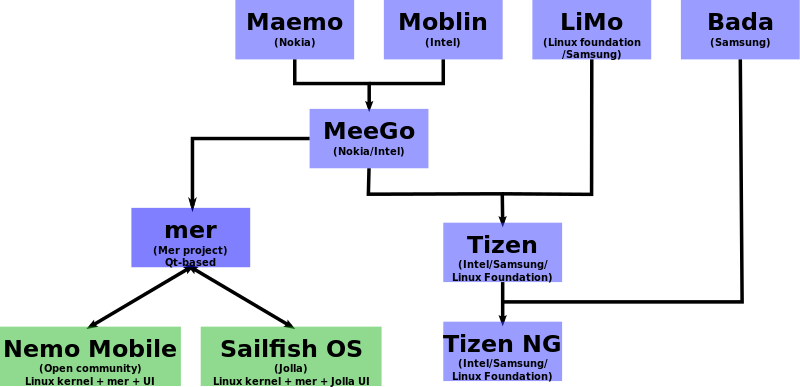
\includegraphics[scale=0.4]{img/cp01/img0103.png}

Existen sistemas operativos móviles basados en linux, que fueron desarrollados bajo el patrocinio de Linux Foundation, algunos de ellos son MeeGo y Tizen que buscaban entrar en 
el mercado global para competir directamente con los grandes SO como Android.

MeeGo surgió de la unión de Nokia y Intel, para crear un sistema operativo basado en linux que además de funcionar en celulares, lo hiciera en Netbooks, sistemas de vehículos y 
televisores, algunos dispositivos como el Samsung N9 lanzado a finales de 2011 contó con este sistema, MeeGo a pesar de seguir activo cuenta con muy pocos usuarios en el mundo.

Tizen fue lanzado en el 2012 producto de de una asociación de grandes empresas, entre ellas Linux Foundation y Samsung, cuenta con una interfaz moderna basada en HTML5 y desde la 
versión 2.2 es compatible con aplicaciones de Android, lo que hace que sea un sistema operativo de gran alcance y con potencial gran cantidad de usuarios.

\subsection*{WebOS}
WebOS fue originalmente creado por Palm Inc. como sucesor de Palm OS para ser un sistema operativo para móviles multitarea, este fue presentado en el 2009 con el Palm Pre, pero 
no tuvo gran acogida en el mercado, en el 2010 cuando Hewlett-Packard compra Palm Inc. renombraron WebOS como HP WebOs, y lanzaron una nueva línea de dispositivos, entre ellos la 
tablet HP TouchPad, pero en 2011 HP anunció que descontinuará sus dispositivos con WebOS, haciendo de WebOS prácticamente un fracaso.

Pero quién supo obtener provecho de este sistema operativo es LG quien en 2013 lo adquirió y lo incorporo como la plataforma de sus nuevos televisores inteligentes, lo que fue un 
gran éxito para LG ya que con este sistema ha logrado vender millones de televisores en el mundo, si bien WebOS originalmente fue orientado a los dispositivos móviles hoy logra 
supremacía en otro rango de dispositivos presentes también en todo el mundo.